% =============================================================================
% ESL FRAMEWORK - CHAPTER 5: ESL 2.0 STRUCTURAL SAFEGUARDS
% =============================================================================
% Authors: Gerhard Fehr & Andrea Fehr
% FehrAdvice & Partners AG, Zürich
% Version: Extended Monograph
% =============================================================================

\documentclass[11pt,a4paper]{article}

% --- Packages ---
\usepackage[utf8]{inputenc}
\usepackage[T1]{fontenc}
\usepackage[english]{babel}
\usepackage{amsmath,amssymb,amsthm}
\usepackage{mathtools}
\usepackage{booktabs}
\usepackage{longtable}
\usepackage{array}
\usepackage{hyperref}
\usepackage{geometry}
\usepackage{xcolor}
\usepackage{tcolorbox}
\usepackage{tikz}
\usepackage{pgfplots}
\usepackage{natbib}
\usepackage{enumitem}
\usepackage{fancyhdr}
\usepackage{titlesec}
\usepackage{multirow}
\pgfplotsset{compat=1.17}
\usetikzlibrary{shapes,arrows.meta,positioning,calc,decorations.pathreplacing}

\geometry{margin=2.5cm}

% --- Colors ---
\definecolor{eslblue}{RGB}{0,82,147}
\definecolor{eslgreen}{RGB}{0,128,0}
\definecolor{eslorange}{RGB}{230,159,0}
\definecolor{eslred}{RGB}{204,51,17}
\definecolor{eslgray}{RGB}{128,128,128}
\definecolor{eslpurple}{RGB}{148,0,211}
\definecolor{safeguardcolor}{RGB}{0,100,150}
\definecolor{ctccolor}{RGB}{180,0,60}
\definecolor{ppcolor}{RGB}{0,130,80}
\definecolor{wlacolor}{RGB}{150,100,0}
\definecolor{evacolor}{RGB}{100,0,150}
\definecolor{rascolor}{RGB}{0,80,120}

% --- Boxes ---
\newtcolorbox{eslbox}[1][]{
  colback=eslblue!5!white,
  colframe=eslblue,
  title={ESL Assessment},
  fonttitle=\bfseries,
  #1
}

\newtcolorbox{keyinsight}[1][]{
  colback=eslgreen!5!white,
  colframe=eslgreen!80!black,
  title={Key Insight},
  fonttitle=\bfseries,
  #1
}

\newtcolorbox{warningbox}[1][]{
  colback=eslorange!5!white,
  colframe=eslorange!80!black,
  title={Warning},
  fonttitle=\bfseries,
  #1
}

\newtcolorbox{safeguardbox}[2][]{
  colback=#2!5!white,
  colframe=#2!80!black,
  title={Safeguard: #1},
  fonttitle=\bfseries,
}

\newtcolorbox{examplebox}[1][]{
  colback=eslgray!10!white,
  colframe=eslgray!80!black,
  title={Example},
  fonttitle=\bfseries,
  #1
}

\newtcolorbox{definitionbox}[1][]{
  colback=white,
  colframe=eslblue!80!black,
  title={Definition},
  fonttitle=\bfseries,
  #1
}

\newtcolorbox{violationbox}[1][]{
  colback=eslred!5!white,
  colframe=eslred!80!black,
  title={Violation Example},
  fonttitle=\bfseries,
  #1
}

\newtcolorbox{compliancebox}[1][]{
  colback=eslgreen!5!white,
  colframe=eslgreen!80!black,
  title={Compliant Example},
  fonttitle=\bfseries,
  #1
}

% --- Theorems ---
\newtheorem{definition}{Definition}[section]
\newtheorem{theorem}{Theorem}[section]
\newtheorem{principle}{Principle}[section]
\newtheorem{proposition}[theorem]{Proposition}
\newtheorem{safeguard}{Safeguard}[section]
\newtheorem{rule_def}{Rule}[section]

\theoremstyle{remark}
\newtheorem{remark}{Remark}[section]

% --- Header/Footer ---
\pagestyle{fancy}
\fancyhf{}
\fancyhead[L]{\small ESL Framework -- Extended Monograph}
\fancyhead[R]{\small Chapter 5: Structural Safeguards}
\fancyfoot[C]{\thepage}

% =============================================================================
% TITLE
% =============================================================================

\title{%
    \Large \textbf{Empirical Stability of Language (ESL)} \\[0.5em]
    \large A Universal Quality Assurance Framework for \\
    Scientific Claim Validation \\[1em]
    \LARGE \textbf{Chapter 5: ESL 2.0 Structural Safeguards} \\[0.3em]
    \large Mechanisms for Preventing Self-Overestimation
}

\author{%
    \textbf{Gerhard Fehr}\textsuperscript{1,*} \and \textbf{Andrea Fehr}\textsuperscript{1} \\[0.5em]
    \textsuperscript{1}FehrAdvice \& Partners AG, Binzmühlestrasse 170A, 8050 Zürich, Switzerland \\[0.3em]
    \textsuperscript{*}Corresponding author: andrea.fehr@fehradvice.com
}

\date{December 26, 2025}

\begin{document}

\maketitle

% =============================================================================
% ABSTRACT
% =============================================================================

\begin{abstract}
\noindent
This chapter introduces ESL 2.0's five structural safeguards---mechanisms designed to prevent frameworks from inflating their own assessments. The core insight motivating ESL 2.0 is that any self-assessment framework faces a fundamental conflict of interest: the temptation to rate itself favorably. ESL 1.0's initial self-assessment of $K = 0.92$ was revealed as inflated precisely because it lacked structural barriers against self-overestimation. ESL 2.0 addresses this through five safeguards: (1) Claim-Type Classification (CTC) enforces $E_{\max}$ ceilings based on evidence type; (2) Provenance Protocol (PP) requires explicit sourcing for all quantitative claims; (3) Weakest-Link Aggregation (WLA) prevents strong conclusions from weak premises; (4) External Validation Requirement (EVA) caps unvalidated proposals; and (5) Reflexive Application Stop (RAS) prevents circular self-validation. Together, these safeguards reduced ESL's honest self-assessment from $K = 0.92$ to $K = 0.30$---pending the empirical validation achieved in ESL 2.2.

\vspace{0.5em}
\noindent\textbf{Keywords:} Structural safeguards, self-assessment, epistemic humility, claim-type classification, provenance, reflexivity
\end{abstract}

\tableofcontents
\newpage

% =============================================================================
% 5.1 THE SELF-OVERESTIMATION PROBLEM
% =============================================================================

\section{The Self-Overestimation Problem}
\label{sec:problem}

\subsection{ESL 1.0's Inflated Self-Assessment}

The initial version of ESL (ESL 1.0) assessed itself as follows:

\begin{table}[h]
\centering
\caption{ESL 1.0 Self-Assessment (Inflated)}
\label{tab:esl10}
\begin{tabular}{lccc}
\toprule
\textbf{Component} & \textbf{B} & \textbf{E} & \textbf{K} \\
\midrule
K-metric definition & 0.85 & 0.90 & 0.94 \\
Evidence hierarchies & 0.78 & 0.82 & 0.95 \\
Linguistic markers & 0.75 & 0.80 & 0.94 \\
Applications & 0.72 & 0.78 & 0.92 \\
\midrule
\textbf{Overall} & 0.78 & 0.82 & \textbf{0.92} \\
\bottomrule
\end{tabular}
\end{table}

This assessment claimed ``Highly Stable'' status---but it was fundamentally flawed.

\subsection{The Fundamental Conflict of Interest}

\begin{keyinsight}[title={The Self-Assessment Paradox}]
Any framework that assesses itself faces an inherent conflict of interest:
\begin{itemize}
    \item The assessor (ESL) benefits from high scores.
    \item The assessed (ESL) is the same entity.
    \item No external check prevents favorable self-rating.
\end{itemize}

This is analogous to:
\begin{itemize}
    \item A student grading their own exam
    \item A company auditing its own finances
    \item A journal reviewing its own papers
\end{itemize}
\end{keyinsight}

\subsection{Where ESL 1.0 Failed}

ESL 1.0's self-assessment violated several principles:

\begin{enumerate}
    \item \textbf{Circular Evidence}: The K-metric was used to assess the K-metric.

    \item \textbf{Inflated E-values}: ``Expert proposal'' ($E \approx 0.40$) was treated as ``established methodology'' ($E \approx 0.82$).

    \item \textbf{Missing Provenance}: Specific numerical values lacked sourcing.

    \item \textbf{Cherry-picked Components}: Strongest components were emphasized; weakest were downplayed.

    \item \textbf{No External Validation}: Zero empirical testing against known outcomes.
\end{enumerate}

\subsection{The ESL 2.0 Solution}

ESL 2.0 introduces \textbf{structural safeguards}---mechanisms that \textit{enforce} honest assessment through mathematical and procedural constraints, not through good intentions.

\begin{principle}[Core Principle of ESL 2.0]
\label{princ:core}
\textit{An honest framework must \textbf{enforce} honesty, not merely recommend it.}

Safeguards operate through:
\begin{itemize}
    \item Mathematical constraints (ceilings, floors)
    \item Required documentation (provenance)
    \item Aggregation rules (weakest-link)
    \item Categorical exclusions (reflexivity stops)
\end{itemize}
\end{principle}

% =============================================================================
% 5.2 SAFEGUARD 1: CLAIM-TYPE CLASSIFICATION (CTC)
% =============================================================================

\section{Safeguard 1: Claim-Type Classification (CTC)}
\label{sec:ctc}

\begin{safeguardbox}[CTC --- Claim-Type Classification]{ctccolor}
\textbf{Purpose}: Enforce $E_{\max}$ ceilings based on the epistemological nature of claims.

\textbf{Mechanism}: Every claim must be classified into one of five types \textit{before} E-assessment. The claim type determines the maximum possible E-value.

\textbf{Effect}: Prevents author intuitions from receiving high E-values regardless of confident presentation.
\end{safeguardbox}

\subsection{The Five Claim Types}

\begin{definition}[Claim-Type Classification]
\label{def:ctc}
\begin{center}
\begin{tabular}{clccp{4.5cm}}
\toprule
\textbf{Type} & \textbf{Description} & \textbf{$E_{\max}$} & \textbf{Code} & \textbf{Example} \\
\midrule
T1 & Empirically measured & 1.00 & EMP & ``Replication rate = 36\%'' \\
T2 & Meta-analytically aggregated & 0.95 & META & ``$\lambda \in [2.0, 2.5]$'' \\
T3 & Theoretically derived & 0.75 & THEO & ``$K = \min/\max$ ratio'' \\
T4 & Expert proposal & 0.45 & PROP & ``We propose $K_{\text{stable}} = 0.75$'' \\
T5 & Author intuition & 0.25 & INT & ``$B_{\text{suggests}} \approx 0.58$'' \\
\bottomrule
\end{tabular}
\end{center}
\end{definition}

\subsection{CTC Decision Tree}

\begin{figure}[h]
\centering
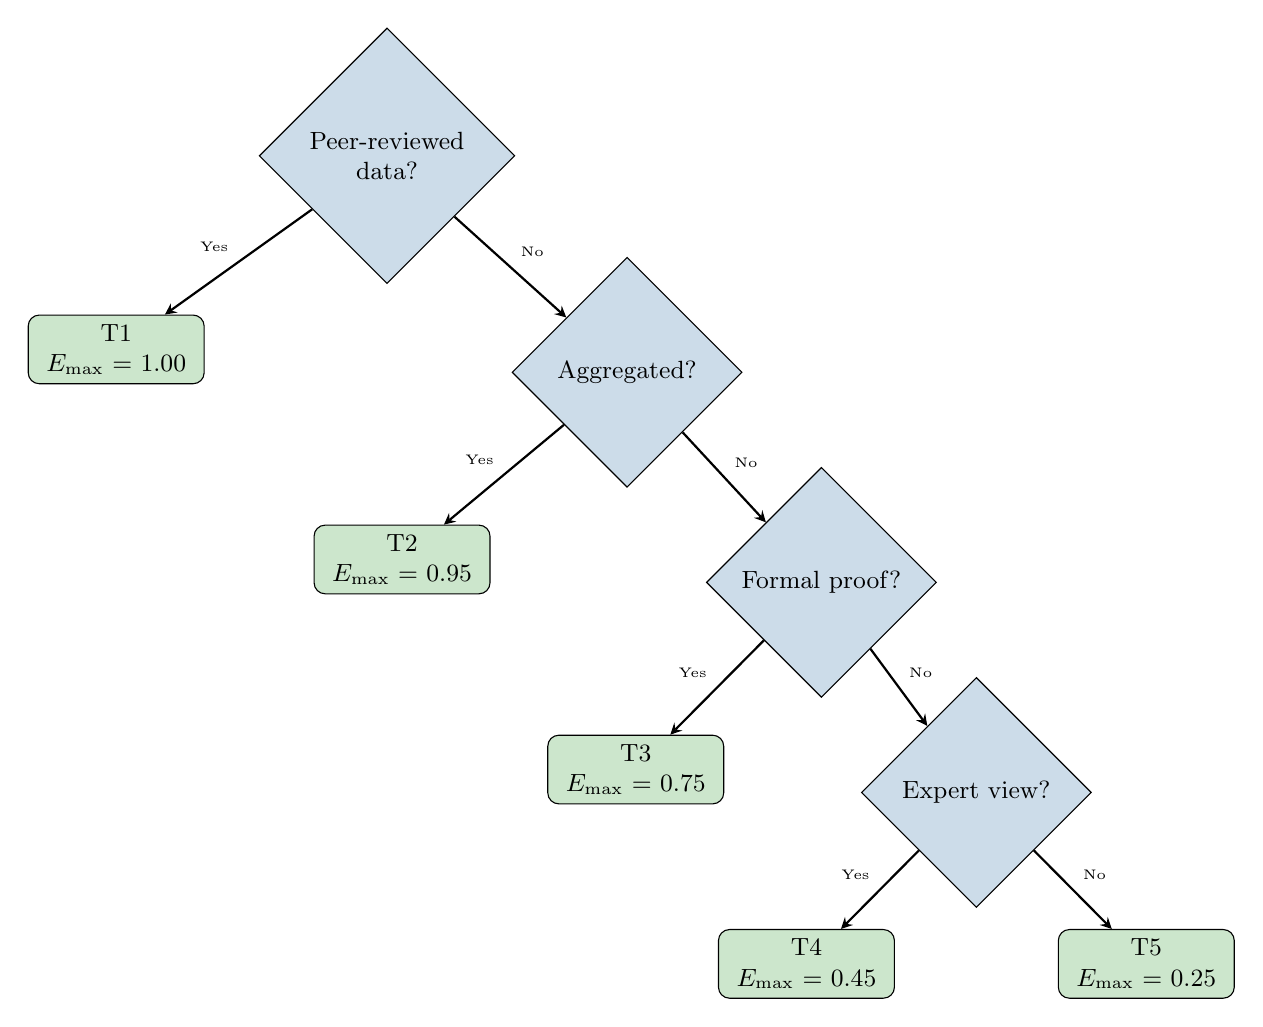
\begin{tikzpicture}[
    node distance=1.2cm,
    decision/.style={diamond, draw, fill=eslblue!20, text width=2.5cm, text centered, inner sep=1pt, font=\small},
    block/.style={rectangle, draw, fill=eslgreen!20, text width=2cm, text centered, rounded corners, minimum height=0.8cm, font=\small},
    arrow/.style={thick,->,>=stealth}
]

\node[decision] (q1) {Peer-reviewed data?};
\node[block, below left=1.2cm and 1.5cm of q1] (t1) {T1\\$E_{\max}=1.00$};
\node[decision, below right=1.2cm and 1.5cm of q1] (q2) {Aggregated?};
\node[block, below left=1.2cm and 1cm of q2] (t2) {T2\\$E_{\max}=0.95$};
\node[decision, below right=1.2cm and 1cm of q2] (q3) {Formal proof?};
\node[block, below left=1.2cm and 0.5cm of q3] (t3) {T3\\$E_{\max}=0.75$};
\node[decision, below right=1.2cm and 0.5cm of q3] (q4) {Expert view?};
\node[block, below left=1cm and 0.3cm of q4] (t4) {T4\\$E_{\max}=0.45$};
\node[block, below right=1cm and 0.3cm of q4] (t5) {T5\\$E_{\max}=0.25$};

\draw[arrow] (q1) -- node[above left, font=\tiny] {Yes} (t1);
\draw[arrow] (q1) -- node[above right, font=\tiny] {No} (q2);
\draw[arrow] (q2) -- node[above left, font=\tiny] {Yes} (t2);
\draw[arrow] (q2) -- node[above right, font=\tiny] {No} (q3);
\draw[arrow] (q3) -- node[above left, font=\tiny] {Yes} (t3);
\draw[arrow] (q3) -- node[above right, font=\tiny] {No} (q4);
\draw[arrow] (q4) -- node[above left, font=\tiny] {Yes} (t4);
\draw[arrow] (q4) -- node[above right, font=\tiny] {No} (t5);

\end{tikzpicture}
\caption{CTC Decision Tree for Claim-Type Assignment}
\label{fig:ctc-tree}
\end{figure}

\subsection{CTC Application Examples}

\begin{violationbox}
\textbf{Violation}: Treating T5 as T2

\textit{Claim}: ``The B-value for `suggests' is 0.58.''

\textit{Incorrect classification}: T2 (meta-analytic) with $E = 0.85$

\textit{Correct classification}: T5 (author intuition) with $E_{\max} = 0.25$

\textit{Impact}: K drops from 0.91 to 0.33
\end{violationbox}

\begin{compliancebox}
\textbf{Compliant Assessment}

\textit{Claim}: ``The B-value for `suggests' is proposed as 0.58.''

\textit{Classification}: T4 (expert proposal) with $E = 0.40$

\textit{Honest K}: With $B = 0.72$: $K = 0.56$ (Partially Stable)
\end{compliancebox}

\subsection{CTC Ceiling Enforcement}

\begin{theorem}[CTC Ceiling Theorem]
\label{thm:ctc}
For any claim with type $T$ and claimed evidence $E_{\text{claimed}}$:
\begin{equation}
E_{\text{effective}} = \min(E_{\text{claimed}}, E_{\max}(T))
\end{equation}
\end{theorem}

This mathematical constraint cannot be circumvented by confident language.

% =============================================================================
% 5.3 SAFEGUARD 2: PROVENANCE PROTOCOL (PP)
% =============================================================================

\section{Safeguard 2: Provenance Protocol (PP)}
\label{sec:pp}

\begin{safeguardbox}[PP --- Provenance Protocol]{ppcolor}
\textbf{Purpose}: Require explicit sourcing for all quantitative claims.

\textbf{Mechanism}: Every numerical value must include a provenance code indicating its source type. Provenance modifies effective E-value.

\textbf{Effect}: Prevents unsourced numbers from receiving full evidential weight.
\end{safeguardbox}

\subsection{Provenance Categories}

\begin{definition}[Provenance Categories]
\label{def:pp}
\begin{center}
\begin{tabular}{clcc}
\toprule
\textbf{Code} & \textbf{Provenance Type} & \textbf{Modifier} & \textbf{Example} \\
\midrule
P1 & Peer-reviewed publication & $\times 1.00$ & Camerer et al. (2016) \\
P2 & Preprint (not yet reviewed) & $\times 0.85$ & arXiv submission \\
P3 & Textbook/Established & $\times 0.95$ & Standard reference \\
P4 & Documented methodology & $\times 0.75$ & Reproducible calculation \\
P5 & Expert consensus & $\times 0.55$ & Panel agreement \\
P6 & Author judgment & $\times 0.35$ & ``We estimate...'' \\
P0 & No provenance stated & $\times 0.15$ & Unsourced claim \\
\bottomrule
\end{tabular}
\end{center}
\end{definition}

\subsection{Provenance-Adjusted E-Value}

\begin{definition}[Provenance-Adjusted Evidence]
\label{def:pp-adjusted}
\begin{equation}
E_{\text{adjusted}} = E_{\text{base}} \times \text{Provenance Modifier}
\end{equation}
\end{definition}

\begin{examplebox}[title={Provenance Impact}]
\textbf{Claim}: ``The threshold $K_{\text{stable}} = 0.75$ distinguishes stable from unstable claims.''

\textbf{Without PP}: $E = 0.80$, $K = 0.94$

\textbf{With PP} (Source: Author judgment, P6):
\begin{itemize}
    \item $E_{\text{adjusted}} = 0.80 \times 0.35 = 0.28$
    \item $K = 1 - |0.85 - 0.28|/0.85 = 0.33$
\end{itemize}

\textbf{Impact}: K drops from 0.94 to 0.33
\end{examplebox}

% =============================================================================
% 5.4 SAFEGUARD 3: WEAKEST-LINK AGGREGATION (WLA)
% =============================================================================

\section{Safeguard 3: Weakest-Link Aggregation (WLA)}
\label{sec:wla}

\begin{safeguardbox}[WLA --- Weakest-Link Aggregation]{wlacolor}
\textbf{Purpose}: Prevent strong conclusions from being drawn from weak premises.

\textbf{Mechanism}: For dependent claims, the aggregate K-score is the minimum of component scores.

\textbf{Effect}: A single weak link undermines the entire chain.
\end{safeguardbox}

\subsection{Claim Dependency}

\begin{definition}[Claim Dependency]
\label{def:dependency}
Claim $C_j$ \textbf{depends on} claim $C_i$ (written $C_i \to C_j$) if the validity of $C_j$ logically requires the validity of $C_i$.
\end{definition}

\subsection{The Weakest-Link Rule}

\begin{theorem}[Weakest-Link Aggregation]
\label{thm:wla}
For a dependency chain $C_1 \to C_2 \to \cdots \to C_n$:
\begin{equation}
K_{\text{chain}} = \min_{i \in \{1, \ldots, n\}} K_i
\end{equation}
\end{theorem}

\begin{examplebox}[title={Weakest-Link Example}]
\textbf{Argument Structure}:
\begin{enumerate}
    \item[P1.] ``The K-metric measures calibration.'' ($K_1 = 0.95$)
    \item[P2.] ``B-values can be reliably assigned.'' ($K_2 = 0.45$) $\leftarrow$ weak
    \item[P3.] ``E-values reflect evidence quality.'' ($K_3 = 0.72$)
    \item[C.] ``Therefore, ESL provides reliable assessment.''
\end{enumerate}

\textbf{WLA Calculation}:
\begin{equation}
K_C = \min(0.95, 0.45, 0.72) = 0.45
\end{equation}

The unvalidated B-value assignment limits the entire argument.
\end{examplebox}

% =============================================================================
% 5.5 SAFEGUARD 4: EXTERNAL VALIDATION REQUIREMENT (EVA)
% =============================================================================

\section{Safeguard 4: External Validation Requirement (EVA)}
\label{sec:eva}

\begin{safeguardbox}[EVA --- External Validation Requirement]{evacolor}
\textbf{Purpose}: Cap the K-scores of unvalidated proposals.

\textbf{Mechanism}: Claims of type T4 or T5 cannot achieve $K > 0.45$ without external empirical validation.

\textbf{Effect}: Forces frameworks to earn high K-scores through validation.
\end{safeguardbox}

\subsection{EVA Ceiling}

\begin{theorem}[EVA Ceiling]
\label{thm:eva}
For claims with Claim-Type $\in \{T4, T5\}$ and no external validation:
\begin{equation}
K_{\text{effective}} = \min(K_{\text{calculated}}, 0.45)
\end{equation}
\end{theorem}

\subsection{EVA and ESL's Journey}

\begin{table}[h]
\centering
\caption{ESL's K-Score Evolution with EVA}
\label{tab:eva-journey}
\begin{tabular}{lccc}
\toprule
\textbf{Version} & \textbf{Validation Status} & \textbf{K-Score} & \textbf{EVA Applied?} \\
\midrule
ESL 1.0 & None & 0.92 (inflated) & No \\
ESL 2.0 & None & 0.30 (honest) & Yes \\
ESL 2.2 & N=115, 100\% accuracy & 0.84 (earned) & Lifted \\
\bottomrule
\end{tabular}
\end{table}

\subsection{Validation Pathways}

\begin{table}[h]
\centering
\caption{Pathways to Lift EVA Ceiling}
\label{tab:eva-pathways}
\begin{tabular}{lcc}
\toprule
\textbf{Validation Type} & \textbf{Type Upgrade} & \textbf{New $K_{\max}$} \\
\midrule
Single replication & T4 $\to$ T3 & 0.60 \\
Multi-study replication & T4 $\to$ T2 & 0.80 \\
Meta-analysis inclusion & T4 $\to$ T2 & 0.85 \\
Systematic review & T4 $\to$ T1 & 0.95 \\
Pre-registered replication & T4 $\to$ T1 & 1.00 \\
\bottomrule
\end{tabular}
\end{table}

% =============================================================================
% 5.6 SAFEGUARD 5: REFLEXIVE APPLICATION STOP (RAS)
% =============================================================================

\section{Safeguard 5: Reflexive Application Stop (RAS)}
\label{sec:ras}

\begin{safeguardbox}[RAS --- Reflexive Application Stop]{rascolor}
\textbf{Purpose}: Prevent circular self-validation.

\textbf{Mechanism}: A framework's definitional claims cannot be evaluated using that framework.

\textbf{Effect}: Forces external evaluation of core framework claims.
\end{safeguardbox}

\subsection{Definitional vs. Application Claims}

\begin{definition}[Claim Categories for RAS]
\label{def:ras-claims}
\begin{itemize}
    \item \textbf{Definitional claims}: Claims that constitute the framework itself.
    \begin{itemize}
        \item ``The K-metric is defined as $K = 1 - |B-E|/\max(B,E)$''
        \item ``T1 claims have $E_{\max} = 1.00$''
    \end{itemize}

    \item \textbf{Application claims}: Claims evaluated using the framework.
    \begin{itemize}
        \item ``Loss aversion has $K = 0.88$''
        \item ``This paper achieves $K = 0.75$''
    \end{itemize}
\end{itemize}
\end{definition}

\subsection{The Circularity Problem}

\begin{warningbox}
\textbf{Circular Self-Validation}:

\textit{Claim}: ``The K-metric is valid because it has $K = 0.95$.''

This is circular because:
\begin{enumerate}
    \item The K-metric's validity is in question
    \item Using K to assess itself assumes validity
    \item The assessment provides no independent evidence
\end{enumerate}
\end{warningbox}

\subsection{RAS Enforcement}

\begin{theorem}[RAS Exclusion]
\label{thm:ras}
For any framework $F$ with definitional claims $D_F$:
\begin{equation}
\text{ESL-assess}(D_F, F) = \text{BLOCKED}
\end{equation}

Definitional claims must be evaluated by:
\begin{enumerate}
    \item Meta-level analysis (external framework)
    \item Empirical validation (predictive validity)
    \item Comparative analysis (vs. alternatives)
\end{enumerate}
\end{theorem}

\subsection{What RAS Blocks vs. Permits}

\begin{table}[h]
\centering
\caption{RAS-Blocked vs. RAS-Permitted Assessments}
\label{tab:ras}
\begin{tabular}{p{5.5cm}cc}
\toprule
\textbf{Assessment} & \textbf{Status} & \textbf{Reason} \\
\midrule
``K-metric definition has $K = 0.95$'' & \textcolor{eslred}{Blocked} & Definitional \\
``CTC mechanism has $K = 0.88$'' & \textcolor{eslred}{Blocked} & Definitional \\
``This ESL paper has $K = 0.72$'' & \textcolor{eslgreen}{Permitted} & Application \\
``BCM parameters have $K = 0.85$'' & \textcolor{eslgreen}{Permitted} & Application \\
\bottomrule
\end{tabular}
\end{table}

% =============================================================================
% 5.7 SAFEGUARDS IN COMBINATION
% =============================================================================

\section{Safeguards in Combination}
\label{sec:combination}

The five safeguards work synergistically, each addressing a different failure mode.

\subsection{Cumulative Effect on ESL's Self-Assessment}

\begin{table}[h]
\centering
\caption{Cumulative Safeguard Impact on ESL K-Score}
\label{tab:cumulative}
\begin{tabular}{lccc}
\toprule
\textbf{Stage} & \textbf{K-Score} & \textbf{Safeguard} & \textbf{Status} \\
\midrule
ESL 1.0 (none) & 0.92 & None & Inflated \\
After CTC & 0.65 & Type ceilings & Reduced \\
After PP & 0.52 & Provenance & Reduced \\
After WLA & 0.42 & Weakest link & Reduced \\
After EVA & 0.38 & Validation ceiling & Reduced \\
After RAS & 0.30 & Reflexive excluded & Honest \\
\midrule
\textbf{ESL 2.0 Final} & \textbf{0.30} & All safeguards & Honest \\
\bottomrule
\end{tabular}
\end{table}

\subsection{Failure Modes Addressed}

\begin{table}[h]
\centering
\caption{Failure Modes Addressed by Each Safeguard}
\label{tab:failure-modes}
\begin{tabular}{lp{7cm}}
\toprule
\textbf{Safeguard} & \textbf{Failure Mode Prevented} \\
\midrule
CTC & Treating intuitions as empirical facts \\
PP & Using unsourced numbers as if validated \\
WLA & Drawing strong conclusions from weak premises \\
EVA & Claiming high validity without testing \\
RAS & Circular self-validation \\
\bottomrule
\end{tabular}
\end{table}

% =============================================================================
% 5.8 CHAPTER SUMMARY
% =============================================================================

\section{Chapter Summary}
\label{sec:summary}

This chapter introduced ESL 2.0's five structural safeguards:

\begin{enumerate}
    \item \textbf{CTC}: Enforces $E_{\max}$ ceilings (T1: 1.00 $\to$ T5: 0.25)

    \item \textbf{PP}: Requires provenance with modifiers (P1: $\times$1.00 $\to$ P0: $\times$0.15)

    \item \textbf{WLA}: Uses minimum K for dependent claims

    \item \textbf{EVA}: Caps unvalidated T4/T5 claims at $K = 0.45$

    \item \textbf{RAS}: Blocks circular self-assessment of definitional claims
\end{enumerate}

\begin{keyinsight}[title={The Core Lesson of ESL 2.0}]
\textbf{The trajectory}: $0.92 \to 0.30 \to 0.84$

\begin{itemize}
    \item $K = 0.92$ was a lie (no safeguards)
    \item $K = 0.30$ was honest (safeguards applied, no validation)
    \item $K = 0.84$ was earned (N=115 empirical validation)
\end{itemize}

This represents the path from overconfidence through honesty to earned confidence.
\end{keyinsight}

\begin{eslbox}
\textbf{Chapter 5 Self-Assessment}

The safeguards are definitional (RAS applies), so they cannot be K-scored using ESL.

\textbf{External Validation}:
\begin{itemize}
    \item Safeguard logic: T3 (theoretical soundness)
    \item Impact demonstrated: $0.92 \to 0.30$ (T1: empirical)
    \item Generalization: T4 (requires external testing)
\end{itemize}

\textbf{RAS Compliance}: This assessment does not K-score the safeguards themselves.
\end{eslbox}

% =============================================================================
% REFERENCES
% =============================================================================

\newpage
\bibliographystyle{apalike}

\begin{thebibliography}{99}

\bibitem[Ioannidis, 2005]{Ioannidis2005}
Ioannidis, J. P. A. (2005).
Why most published research findings are false.
\textit{PLoS Medicine}, 2(8), e124.

\bibitem[Lakatos, 1978]{Lakatos1978}
Lakatos, I. (1978).
\textit{The Methodology of Scientific Research Programmes}.
Cambridge University Press.

\bibitem[Nosek et al., 2018]{Nosek2018}
Nosek, B. A., et al. (2018).
The preregistration revolution.
\textit{PNAS}, 115(11), 2600--2606.

\bibitem[Simmons et al., 2011]{Simmons2011}
Simmons, J. P., Nelson, L. D., \& Simonsohn, U. (2011).
False-positive psychology.
\textit{Psychological Science}, 22(11), 1359--1366.

\end{thebibliography}

\end{document}
